\documentclass[journal]{vgtc}                % final (journal style)
%\documentclass[review,journal]{vgtc}         % review (journal style)
%\documentclass[widereview]{vgtc}             % wide-spaced review
%\documentclass[preprint,journal]{vgtc}       % preprint (journal style)
%\documentclass[electronic,journal]{vgtc}     % electronic version, journal

%% Uncomment one of the lines above depending on where your paper is
%% in the conference process. ``review'' and ``widereview'' are for review
%% submission, ``preprint'' is for pre-publication, and the final version
%% doesn't use a specific qualifier. Further, ``electronic'' includes
%% hyperreferences for more convenient online viewing.

%% Please use one of the ``review'' options in combination with the
%% assigned online id (see below) ONLY if your paper uses a double blind
%% review process. Some conferences, like IEEE Vis and InfoVis, have NOT
%% in the past.

%% Please note that the use of figures other than the optional teaser is not permitted on the first page
%% of the journal version.  Figures should begin on the second page and be
%% in CMYK or Grey scale format, otherwise, colour shifting may occur
%% during the printing process.  Papers submitted with figures other than the optional teaser on the
%% first page will be refused.

%% These three lines bring in essential packages: ``mathptmx'' for Type 1
%% typefaces, ``graphicx'' for inclusion of EPS figures. and ``times''
%% for proper handling of the times font family.

\usepackage{mathptmx}
\usepackage{graphicx}
\usepackage{times}

% \usepackage{egweblnk}
% \usepackage{cite}
\usepackage[color=yellow!30]{todonotes}
\usepackage{color,soul}
\usepackage{multirow}

%% We encourage the use of mathptmx for consistent usage of times font
%% throughout the proceedings. However, if you encounter conflicts
%% with other math-related packages, you may want to disable it.

%% This turns references into clickable hyperlinks.
\usepackage[bookmarks,backref=section,linkcolor=black]{hyperref} %,colorlinks
\hypersetup{
  pdfauthor = {},
  pdftitle = {},
  pdfsubject = {},
  pdfkeywords = {},
  colorlinks=true,
  linkcolor= black,
  citecolor= black,
  pageanchor=true,
  urlcolor = black,
  plainpages = false,
  linktocpage
}

 \usepackage{epstopdf}
%% If you are submitting a paper to a conference for review with a double
%% blind reviewing process, please replace the value ``0'' below with your
%% OnlineID. Otherwise, you may safely leave it at ``0''.
\onlineid{0}

%% declare the category of your paper, only shown in review mode
\vgtccategory{Research}

%% allow for this line if you want the electronic option to work properly
\vgtcinsertpkg

%% In preprint mode you may define your own headline.
%\preprinttext{To appear in an IEEE VGTC sponsored conference.}

%% Paper title.

\title{A Task Taxonomy to support Visualization for the Effective Analysis of Biological Pathways}

%% This is how authors are specified in the journal style

%% indicate IEEE Member or Student Member in form indicated below
\author{Author One and Author Two}
% \authorfooter{
% %% insert punctuation at end of each item
% \item
%  Roy G. Biv is with Starbucks Research. E-mail: roy.g.biv@aol.com.
% \item
%  Ed Grimley is with Grimley Widgets, Inc.. E-mail: ed.grimley@aol.com.
% \item
%  Martha Stewart is with Martha Stewart Enterprises at Microsoft
%  Research. E-mail: martha.stewart@marthastewart.com.
% }

%other entries to be set up for journal
\shortauthortitle{Our short title goes here}
%\shortauthortitle{Firstauthor \MakeLowercase{\textit{et al.}}: Paper Title}

%% Abstract section.
\abstract{
Understanding complicated networks of interactions and chemical components is essential to solving contemporary problems in modern biology, especially in domains such as cancer and systems research.
In these domains, biological pathway data is used to represent chains of interactions that occur within a given biological process.
Visual representations can help researchers understand and interact with complex pathway data in a number of ways.
Biological data sets offer unique challenges for visualization, due to their complexity and heterogeneity.

Here, we present taxonomy of tasks -- generated from interviews with several domain experts -- that are regularly performed by researchers who work with biological pathway data.
These tasks require further classification than is provided by existing taxonomies.

\todo[inline]{more here about how these tasks are different from previous work}

We also examine the existing visualization techniques which support each of the tasks, and we discuss gaps in the existing visualization space revealed by our taxonomy.
We conclude by suggesting future research directions based on our taxonomy and motivated by the comments received by our domain experts.
} % end of abstract

%% Keywords that describe your work. Will show as 'Index Terms' in journal
%% please capitalize first letter and insert punctuation after last keyword
\keywords{Index Terms need to go here}

%% ACM Computing Classification System (CCS).
%% See <http://www.acm.org/class/1998/> for details.
%% The ``\CCScat'' command takes four arguments.

% \CCScatlist{ % not used in journal version
%  \CCScat{K.6.1}{Management of Computing and Information Systems}%
% {Project and People Management}{Life Cycle};
%  \CCScat{K.7.m}{The Computing Profession}{Miscellaneous}{Ethics}
% }

%% Uncomment below to include a teaser figure.
 %  \teaser{
 % \centering
 % \includegraphics[width=16cm]{figures/teaser}
 %  \caption{In the Clouds: Vancouver from Cypress Mountain.}
 %  }

%% Uncomment below to disable the manuscript note
%\renewcommand{\manuscriptnotetxt}{}

%% Copyright space is enabled by default as required by guidelines.
%% It is disabled by the 'review' option or via the following command:
% \nocopyrightspace

%%%%%%%%%%%%%%%%%%%%%%%%%%%%%%%%%%%%%%%%%%%%%%%%%%%%%%%%%%%%%%%%
%%%%%%%%%%%%%%%%%%%%%% START OF THE PAPER %%%%%%%%%%%%%%%%%%%%%%
%%%%%%%%%%%%%%%%%%%%%%%%%%%%%%%%%%%%%%%%%%%%%%%%%%%%%%%%%%%%%%%%%

\begin{document}

%% The ``\maketitle'' command must be the first command after the
%% ``\begin{document}'' command. It prepares and prints the title block.

%% the only exception to this rule is the \firstsection command
%%\firstsection{Introduction}

\maketitle

%% \section{Introduction} %for journal use above \firstsection{..} instead

\section{Introduction}

Understanding complicated networks of bio-molecular interactions and chemical components is essential to solving contemporary problems in modern biology, especially in domains such as cancer and systems research~\cite{hanahan2011hallmarks}.
These bio-molecular interactions are represented in the form \emph{pathways}, which are used to describe a chain of interactions between biochemical and biological entities within a cell.
Pathways are small, curated subsets of a much larger, complex graph of interactions between molecules, and a given pathway usually represents a particular biological process that is relevant within some research context.

Pathways are modeled as entities , relationships and meta-data.
An entity is a component of a pathway such as a gene, a gene product (i.e. a protein), a complex of proteins, a small biomolecule within a cell, or even another pathway.
Relationships between entities can be directed or undirected, can involve more than two entities, and they can represent many different types of biological relationship.
Meta-data can include attributes resulting from experimental data, provenance information (links to related publications), and links to additional resources related to the entity or relationship.
% In order to limit the scope of their analyses...
For example, Figure \ref{fig:kvik} shows a typical representation of a pathway as a human-curated node-link diagram, where nodes are biological entities and edges represent interactions between them.

\begin{figure}[htb]
  \centering
  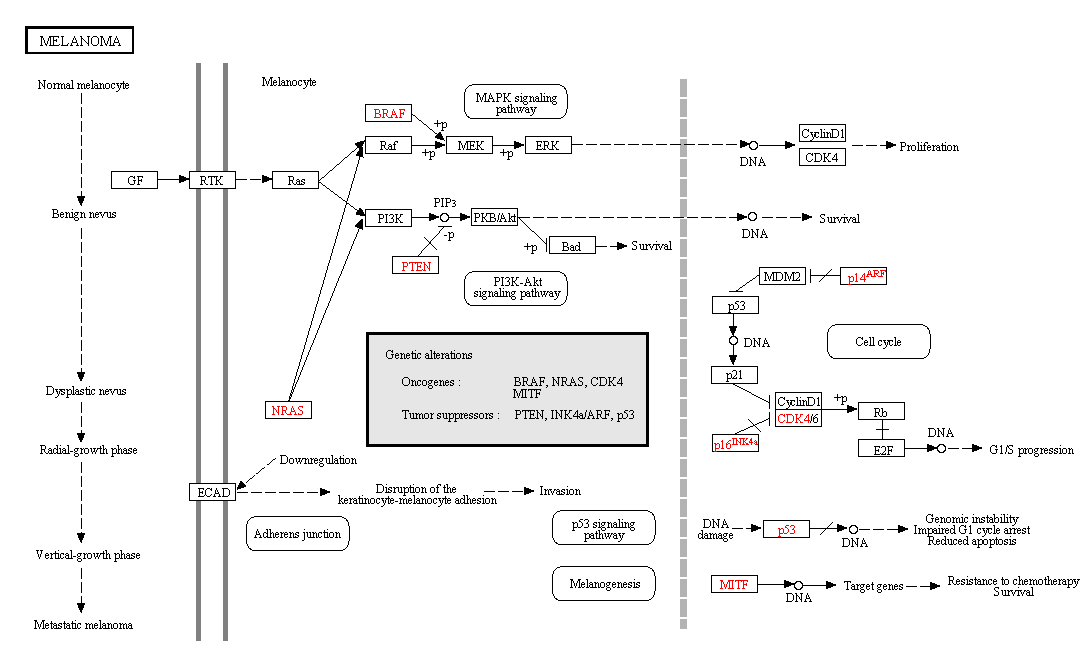
\includegraphics[width=\linewidth]{figures/kegg2}
  \caption{\label{fig:kvik} A view of a typical KEGG diagram. From~\cite{Fjukstad2014kvik}.}
\end{figure}

%\p{Pathways are very complex}

Researchers who work with pathway data are confronted with a number of challenges.
Pathway files may contain hundreds of proteins and biomolecules that participate in a variety of reactions.
In an abstract sense, reactions can be seen as state transitions with multiple inputs and outputs.
Participants --- genes, proteins, and other molecules within a cell --- can act as inputs or outputs to multiple reactions, and the relationships between reactions inherently include feedback loops.
Reactions often have an effect on other reactions, inhibiting or promoting their frequency.
These molecular activation pathways are inherently dynamic, which limits the utility of any static graph representation \cite{kitano2002systems}.
Representing complexity while also enabling researchers to see higher order patterns is a significant challenge \cite{saraiya2005visualizing}.

%\p{Pathways are useful for presentation}

Pathway diagrams can be useful for both presentation and analysis.
For presentation, pathway diagrams can contextualize a set of biological processes within a cell, and diagrams often show the location of cellular membranes in order to help provide a frame of reference for a given process.
Ideally, a pathway diagram allows a viewer to efficiently understand a complex set of biological relationships.

%\p{Pathways are useful for analysis}

While pathways may be useful for presenting and contextualizing a set of reactions, they can also be an important part of analyses in domains related to molecular biology and systems research, among others.
%\p{Domain context}

For example, molecular activation pathways are of critical importance to cancer researchers, who hope to understand --- and potentially disrupt --- malignant cycles of uncontrolled cellular growth, replication, and mediated cell death \cite{cairns2011regulation}.
Effective cancer drug development involves determining how proteins affected by a drug in turn affect important cellular pathways, and in this domain the downstream consequences of a particular drug effect are especially important \cite{luo2003targeting}.
In a separate domain, stem-cell researchers work with pathways that will precipitate a desired cellular differentiation into specific cell types \cite{reya2001stem}.

%\p{Static representations are not enough}

In the last decade, analyses that involve hundreds or thousands of genes and gene products have become common.
When analyzing such large and complex data, visual representations can be essential.
Often, static representations are inadequate.
The complexity and amount of information that needs to be incorporated in given diagram can make static representations cluttered and difficult to interpret.
Thus, modern tools make careful use of user interactions and visualization techniques to allow a user to effectively explore and analyze pathway data.

%\p{Designing effective tools}

Designing effective visual analytics applications requires a detailed understanding of analysis tasks that are performed by the user.
Pathway data are often large and complex, and analysts will want to perform a variety of tasks depending on their research domain.
Tasks may be exploratory in nature, and a useful visualization of pathway data could reveal new insights to a researcher.
Tasks may also involve detailed queries or calculations of various network metrics, for example.
A comprehensive understanding of tasks performed by domain researchers in a typical analysis is essential to the design and implementation of an effective visual analytics application.

%\p{Other reviews}

%Here we perform a comprehensive analysis of tasks and requirements in an effort to design effective platforms for visual analytics of pathway data.
%Previous reviews of pathway analysis tools~\cite{Gehlenborg2010omics,Suderman2007tools} have surveyed the population of available applications.
%However, the most recent review was published over five years ago, and it includes only a surface-level discussion of tasks, requirements, and visual encoding techniques.

%\p{In this work}

In this work, we present a description and analysis of tasks and requirements related to biological pathway research.
Tasks were gathered from several interviews with domain experts who work with biological pathway data.
After an introduction to the structure and content of pathway data, we describe the tasks that were garnered from our interviews.
%Using these tasks, we then describe the high-level requirements of an effective visual analytics platform for pathway data.
We then review visual representations of pathway data in the context of our requirements.
We also review existing tools that implement those visual representations.
Finally, avenues of future research are considered, along with a brief summary of lessons learned from domain experts.



%\subsection{Pathway data}
%
%In order to aid an understanding of pathway visualization tools, an understanding of the structure of pathway data structures is necessary.
%In this section we briefly explain the structure of typical pathway data files.
%
%\subsubsection{Pathway Data Model}
%\todo[inline, author=FMG, color=green]{Is it ok if i condense this subsubsection into a line or two and then move it with the pathway formats subsection , to the related work section?}
%
%Information stored in any pathway data file can generally be broken down into three components:
%
%\begin{itemize}
%
%\item \textbf{Entity}\\
%An entity is a component of a pathway such as a gene, a gene product (i.e. a protein), a complex of proteins, or a small biomolecule within a cell.
%Entities are identified by name and are involved in one or more relationships.
%Importantly, pathways themselves can be entities within other pathways.
%\item \textbf{Relationship}\\
%A relationship involves two or more entities.
%Various kinds of relationships which different biological meanings are present in a pathways.
%Relationships can be directed or undirected, and they can involve more than two entities (meaning the resulting network is a hyper-graph).
%\item \textbf{Meta-data}\\
%The complex nature of the information stored in a pathway requires additional data to be stored with each entity and relationship.
%Meta-data can include experimental data, scientific information such as the molecular structure of a chemical compound, as well as links to additional resources or publications related to an entity or relationship.
%
%\end{itemize}



%-------------------------------------------------------------------------
\section{Related Work}
%-------------------------------------------------------------------------
\subsection{Biological Pathway Visualization}
%\todo[inline]{Need more here on history and importance}


%High throughput techniques have resulted in experiments producing vast amounts of highly complex data.
Pathways models are an important concept with biological research~\cite{cairns2011regulation, luo2003targeting,reya2001stem}.
The complexity of the data and the benefits offered to researchers by visualization tools make biological pathways an important application domain for visualization.


There are a large number of tools available and many existing surveys describe them \cite{Suderman2007tools,pavlopoulos2008survey,Gehlenborg2010omics}.
In this paper we highlight examples of prominent existing tools and techniques which provide support for the tasks described in our taxonomy, however it is not intended as a complete survey of biological visualization applications.
We have included the following: \textit{ChiBe}~\cite{Babur2010chibe}, \textit{Entourage}~\cite{Lex2013entourage}, \textit{Reactome Pathway Browser}~\cite{croft2014reactome}, \textit{VisAnt}~\cite{hu2004visant}, \textit{MetaViz}~\cite{bourqui2007metabolic}, \textit{VitaPad}~\cite{holford2005vitapad}, and \textit{BioFabric}~\cite{Longabaugh2012biofabric}.
It is clear from the relationship structure of pathway data that graphs are a suitable visualization choice, and each of these applications visualizes pathway data as node-link graph representations (or a slight variant in the case of Biofabric~\cite{Longabaugh2012biofabric}.
However, there are alternative visualization techniques which could be applied to pathway data.
Research has shown that matrix visualization techniques outperform node-link diagrams for higher level group based tasks\cite{Ghoniem2004,Henry2007}.
While matrix tasks are not as effective for path-tracing tasks, a juxtaposition of both types or a hybrid visualization hybrid, such as NodeTrix~\cite{NodeTrix2007}, could prove effective.
% mention Set visualization




\subsubsection{Pathway Data Formats}
Pathway data can be stored in one of several file formats.
In particular, \textit{BioPAX}~\cite{demir2010biopax}, \textit{KEGG}~\cite{kanehisa2000kegg} and \textit{SBML} \cite{Hucka2003} are the most popular standards for storing the complex data structures described in the previous section.

These formats are XML-based and represent data as an ontology.
\emph{BioPAX}, in particular, was designed to be a general format for biological pathways across a variety of domain contexts~\cite{demir2010biopax}.
Systems Biology Graph Notation (SBGN)~\cite{Novere2009} is a visual standard often used to visualize \textit{BioPAX} and \textit{SBML} file formats.
This standard defines multiple edge and node types, as well as allowing edges to connect to more than 2 nodes, resulting in a hypergraph visualization.
Other formats are employed for the visualization of biological pathways that are not specific to the field of biology.
For instance \textit{SIF Simple Interaction Format} used by \textit{Cytoscape}~\cite{Shannon2003cytoscape} is used to visualize undirected interactions between participants.

%However, the most recent review was published over five years ago, and it includes only a surface-level discussion of tasks, requirements, and visual encoding techniques.



%-------------------------------------------------------------------------
\subsection{Task Taxonomies}
The field of visual analytics has produced a number of \textit{task taxonomies}, which are written in an effort to understand exactly how various analytics tasks are enabled by different visualization techniques, and vice-versa.
These taxonomies help clarify the utility of existing techniques while also providing a low level template for the design and evaluation of new techniques.
Wehrend and Lewis~\cite{Wehrend1990} provide one of the earliest visualization task taxonomies, with the goal of ``accelerating progress in scientific visualization'' by allowing researchers to easily find the right visualization technique for a given problem.
Schneiderman~\cite{Shneiderman1996} define a ``task by data type taxonomy'' for information visualization in order to \textit{``to sort out the prototypes and guide researchers to new opportunities''}.
These seminal taxonomies were, like many later taxonomies, independent of a specific visualization application domain, their purpose was to provide a low level description and categorization of the analysis tasks enabled by \textit{any} visualization of data.

Later taxonomies focus specifically on more narrow categories of visualization.
For instance, Valiati et al.~\cite{Valiati2006} provide a taxonomy focused specifically on multidimensional visualizations. They build on~\cite{Wehrend1990}, but focus on tasks uniquely related to multidimensional visualizations (such as parallel coordinates).
Like previous authors, their goal is to guide the choices of visualization and interaction techniques, and also to  help support usability testing.
Lee at al~\cite{Lee2006} define a graph visualization taxonomy of tasks that are frequently encountered when analyzing graph data.
The stated goal of this work was to improve the evaluation of graph visualization systems by creating a set of common benchmark tasks (which could be used in conjunction with benchmark data sets).
Their taxonomy covers tasks for the analysis of graphs in general, and was inspired by example tasks from many domains that make regular use of graph data.
The authors build on Amar and Stasko's~\cite{Amar2005} low level visual analytic task list by composing existing low level tasks into higher level complex tasks while also proposing additional tasks that are not captured by low level tasks presented in existing taxonomies.


Several recent taxonomies focus on aspects of graph visualization that extend the work of Lee at al~\cite{Lee2006}.
Ahn et al~\cite{Ahn2014} provide a task taxonomy for analyzing networks that evolve over time, also known as dynamic graphs.
The dynamic and complex nature of dynamic graph data yields a similarly complex set of analysis tasks, and many of these tasks are not covered by the general graph taxonomy of Lee at al~\cite{Lee2006} -- thus, new tasks need to be specified.
Pretorius et al~\cite{Pretorius2014} focus on multivariate graph visualization (where graph elements contain multiple attributes).
Their work builds on the work of both Lee at al~\cite{Lee2006} and of Valiati et al.~\cite{Valiati2006}, as multivariate networks can be considered a multidimensional data set.

The earliest visualization taxonomies were written as very general classifications of low level analytic tasks related to any data visualization.
In more recent publications, and as visualization research has progressed, task taxonomies have increasingly focused on more constrained subsets of tasks related to particular types of data structures.

While recently-published task taxonomies have focused on particular data structures (or for datasets with particular characteristics), to our knowledge this is the first written in the context of the domain of biological pathway analysis.

\todo[inline]{One could argue that the whole point of a taxonomy is to be general, and to ignore domain. We should highlight the benefits of writing a taxonomy based on domain-specific tasks. Or how this interesting... etc.}

Biological Pathway visualization is a complex application domain that poses many specific challenges not encountered in the created of the previous taxonomies
The underlying data sets are dynamic multivariate hyper-graphs, and are more complex than any of those described in previous taxonomies.
The tasks to be completed by biologists are also highly complex, involving many different entity and relationship types, and are not fully covered by the existing taxonomies.
\todo[inline]{Need to demonstrate 100 percent that this is true in the rest of the paper}
%Amar and stasko do include correlation as one of their tasks
% pretorius also includes causation...

%-------------------------------------------------------------------------

\section{Interviews}

Interviews were conducted with seven biological scientists, each of whom works with pathway data in some form.
Those interviewed included one tenured professor, three assistant professors, one researcher at a cancer research institution, one postdoctoral research associate, and one masters student in bioinformatics.
Interviews were loosely structured, but interview questions were designed to elicit a detailed understanding of the tasks performed by the researcher in a typical analysis, as well as an understanding of the type and structure of data that each researcher worked with.
Each researcher also presented their views on the utility of pathway data and pathway diagrams in general.

%-------------------------------------------------------------------------
\section{Task Taxonomy}

\begin{table*}
  \begin{tabular}{| l | l |}
    \hline
    \multirow{2}{*}{Attributes} & Provenance \\
    & Uncertainty \\ \hline
    \multirow{5}{*}{Relationships} & Directed \\
    & Hierarchical \\
    & Compound \\
    & Cascading \\
    & Feedback Loops \\ \hline
  \end{tabular}
\end{table*}

\subsection{Taxonomy Overview}

Biological pathways are generally represented as weighted, directed graphs and in some cases include hyper-edges and compound nodes.
Task taxonomies have been created which describe tasks related to graphs in general. However, the analysis of biomolecular interaction networks includes a unique set of tasks that refine and extend the tasks associated with the visual analysis of networks in general.

\subsection{Attributes}


Most applications provide access to the attributes through simple interactions (e.g. mouseover and click). In many cases the attribute information is simply read from an input file, however more recent tools such as \textit{SBGNViz}~\cite{SBGNViz2015} and \textit{ChiBE}\cite{Babur2010chibe} query online database to provide a range of important attribute information.
The low-level identification of nodes, edges, and their attributes is an essential component in the visual analysis of any graph representation. For biological pathqway visualization in particular, integration of attribute data from external data source is very important.

\subsubsection{Multivariate data visualization} % need better title for subsection
Biological pathways  contain many different attributes that affect the state of a biological entity. 
For example a gene may be up regulated or down regulated under different experimental conditions. 
This change in attributes may be time based (meaning the graph is dynamic) or it may be as a result of the context in which a pathway is being analyzed (e.g. as part of a cancer research study).
Data entities containing multiple attributes are often referred to as multivariate.

 
Multivariate network visualization is a highly active field of visualization, in which the life sciences in general are frequent application domain, see \cite{} for a recent state of the art survey. 
Many more recent  biological network visualizations include attribute information.
CHiBE \textit{ChiBE}\cite{Babur2010chibe} provides the ability to load in biological entity regulation data mappings from an external source and apply them to a pathway visualization.
The most prominent data format for supporting this is the SIF format defined as part of the Cytoscape application \cite{Shannon2003cytoscape}. 
The \textit{RenDoI} application \cite{Vehlow2015}, a plug-in for \textit{Cytoscape} that is used to visualize  biological data knowledge networks uses Degree of Interest functions to highlight nodes based on attribute values.
Such functionality could easily be extend to biological pathway visualizations.
The general purpose visualization system , \textit{Candid} \cite{Shadoan2013}, also uses attribute information as part of hyper graph query system which allows users to perform complex queries on entities of different types.
Node and edge attributes are also used for graph querying and filtering as came be seen in , what is termed \textit{facet} based visualization. This approach allows for graphs to be filtered by subsets of attributes.

\todo[inline]{need to include Cerebral application here}
%To Be Completed

\subsubsection{Provenance}

Especially important to researchers in the field of bioinformatics is the concept of \textit{data provenance}, which refers to the history of original sources tied to a particular entity. Much of the data in the field of bioinformatics is gathered and integrated from a wide range of publications, data stores, and other products of research.
While \textit{SBGNViz}~\cite{SBGNViz2015} and \textit{ChiBE}\cite{Babur2010chibe} and other applications allow connectivity to external sources, such as UNitProt or TBA, provenance information is not visualized directly.

% Does it need to be
\todo[inline] {Discuss Visualization of provenance}

\subsubsection{Uncertainty}

Related to the task of identifying data provenance is the task of being able to view and identify information related to the \textit{uncertainty} of the data underlying relationships between entities.

In interviews, researchers discussed the importance of understanding \emph{uncertainty} within pathway data. For example, each relationship within a BioPAX file is usually associated with a publication that provides evidence for its existence. Thus, some relationships may be subject to scrutiny within the scientific community, while others may have more robust empirical support.

Some databases such as STRING~\cite{STRING2005} , a protein interaction database, provide quality scores with their results. This quality score can be seen as a form of uncertainty based on the provenance of the data.
The higher the score, the more evidence there is for an interaction.

\subsection{Relationships}

Understanding how pathway entities are connected was of critical importance to all of the researchers we interviewed, and is essential to most research in bioinformatics.

\subsubsection{Directed Relationships}

While some analyzes and datasets involve undirected relationships between genes or gene products, studies of metabolic networks and other inter-cellular processes rely on directed relationships, and several researchers that we interviewed stressed the importance of understanding directed relationships between entities.


\begin{figure}[htb]
  \centering
  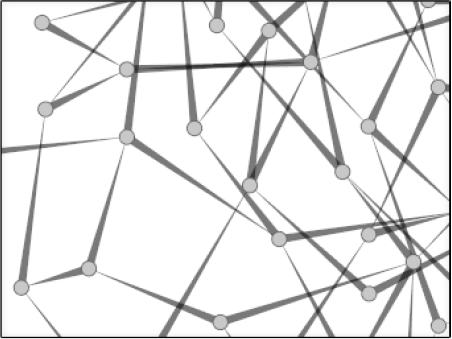
\includegraphics[width=0.5\columnwidth]{figures/tapered_edges}
  \caption{\label{fig:tapered_edges} The tapered directional edges, taken from~\cite{Holten2009}. Permission to be obtained. The narrow end of the edge indicates the target.}
\end{figure}
Many visualization applications use the more traditional approach of arrowheads to indicate edge directions, however work by Holten and van Wijk~\cite{Holten2009} shows that tapered edges (see fig \ref{fig:tapered_edges}) perform more effectively in conveying edge direction. The graphs used in Holten and van Wijk's were simple directed graphs. Biological pathways are usually modeled as hyper-graphs, with many different types of edge and hyper-edge. Visual encodings such as SBGN and KEGG (see figure \ref{fig:kvik}) contain many different visual representations for edges, so applying the tapered edge visualization style to complex biological pathways is not trivial and would require an empirical evaluation. However, the results of Holten and van Wijk's work suggest that investigating such an approach may be worthwhile.


\subsubsection{Hierarchical Relationships}

Pathway data is inherently hierarchical.
Hierarchical relationships describe relationships of containment, and these relationships can be abstract or based on real biochemical interactions within a cell.
For example, a pathway (itself an abstraction) can be nested within other pathways.
These nested pathways generally encapsulate some commonly-understood hierarchy of biological processes that take place within a cell, such as cellular replication.
Other representations include the more general notion of a ``module'' of connected components, such as gene products.
Hierarchical relationships can also represent physical interactions between biochemical participants.
A common of example of this is in bio-molecular complexes, which are themselves composed of other complexes or biomolecules.

It is important to note that hierarchy and ``structure'' often co-exists with other types of relationships. In most cases, pathway data includes relationships of hierarchy (i.e., when one vertex is contained within another) \textit{in parallel} with other, non-hierarchical relationships, such as the relationship between one gene product that activates or inhibits another. Also, note that while non-hierarchical relationships can take a variety of forms, the only form of hierarchical relationship is one of \textit{containment}, from parent to child, and is undirected.

In terms of visualization there are many techniques for showing hierarchical data.
There are many hierarchical tree based graph layouts that position nodes to emphasis hierarchical nature of data, however these are often not suitable for biological pathway layout as the constrains on position in a layout affect the readability of the lowest level of information.
The RenDoI application allows for multiple data sources to be included in a single diagram. 
This may include data from different pathways and is a containment relationship. Essential the node for each data source forms a set, which may or may not overlap with other sets.  
This is visualized using by drawing a bounded contour around the nodes in the set. Different border colors indicate different sets.
This type of encoding of  set membership is the \textit{Bubblesets}~\cite{Collins2009} approach, which was shown to be the most effective way of displaying group information on a node link diagram by Jianu et al.~\cite{Jianu2014}.
\todo[inline]{consider moving previous paragrap to compound Relationships section}


\begin{figure}[htb]
  \centering
  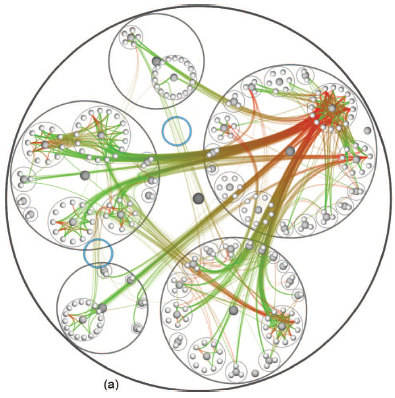
\includegraphics[width=0.5\columnwidth]{figures/Hierarchical_edge_bundles}
  \caption{\label{fig:Hierarchical_edge_bundles} Hierarchical edge bundles, taken from~\cite{Holten2006}. Permission to be obtained. The bundles not only reduce clutter but also more cleary define the hierarchy.}
\end{figure}

In many cases for pathway visualization the hierarchy is not very deep and edges do not traverse multiple levels of the hierarchy.
However in cases where edges do traverse  multiple hierarchical levels they may cause clutter.
Hierarchical Edge Bundling \cite{Holten2006} is a clutter reduction technique, which also emphasizes the hierarchical nature of relationships, see figure\ref{fig:Hierarchical_edge_bundles}. There are many edge bundling techniques in general
}

\subsubsection{Compound Relationships}

A vertex that contains other entities can be represented as a \textit{compound node}, which is equivalent to a ``parent'' vertex or in some contexts a ``module.''

It is important to note that a one-to-one relationship between an entity and a parent is \textit{not} the same as a one-to-many relationship between an entity and all of that parents children.
For instance, BioPax data contains the abstract ``NextStep'' relationship, which defines, as the name suggests, an arbitrary notion of the ``next step'' of some biological process.
A biochemical reaction could be connected, via a \textit{single} ``NextStep'' relationship, to an entire pathway, which could potentially contain thousands of nodes.
This relationship is clearly not the same as a biochemical reaction being connected to every entity within a pathway.

\subsubsection{Causality and Cascading Effects}

\todo[inline, author=PM]{Should we separate discussion of cause and effect from discussion of cascading effects?}

\todo[inline, author=FMG]{I think it would be a good idea to differentiate this taxonomy from Ahn's taxonomy in this section. He does look at causal tasks and repetition, which are related to feedback loops , but not the same....}

A category of tasks inherent to a variety of work in bioinformatics is the identification of \textit{causal relationships} that exist between bio-molecular entities.
When discussing directed paths between entities, one entity is said to be \emph{upstream} or \emph{downstream} of another.

Understanding these upstream and downstream relationships is particularly important to domains such as cancer drug research, where a drug may affect a small subset of genes or gene products, which in turn will affect various downstream processes.
\emph{Causal networks} are also particularly essential to the analysis of large-scale gene expression data.
For instance, a causal network could reveal the likely regulators of a set of genes that are observed to be up-regulated or down-regulated in a particular setting~\cite{felciano2013predictive, Kramer2013ipa-causal}.

In most cases, a directed relationship is meant to represent a biochemical reaction, where one entity is consumed as a reactant and another is produced as a product.
Thus, an upstream entity may be connected to a downstream entity through a chain of several directed links.
In the most basic sense, the ``entities'' mentioned above are genes, gene products (such as proteins or complexes), or other small molecules within a cell.
A researcher may be interested in understanding the path of reactions (or other relationships) that connects two entities.

\subsubsection{Many-to-Many Cascading Effects}

A causal effect may be modeled as a simple directed edge.

\todo[inline, author=PM]{What really matters in biology is determining cause and effect relationships between many sources and many sinks, separated by many other sets of connections}

\subsubsection{Feedback Loops}

Feedback loops are common within metabolic activation networks, and they play a key role in processes related to uncontrolled cellular growth in cancerous cells.

\subsection{Comparisons}

\todo[inline, author=FMG]{Need to add in description of comparison tasks}



In their 2011 survey Gleicher et al. \cite{Gleicher2011} describe three primary types  classifications of comparative visualization. 
These are  juxtaposition, superposition,  and explicit encoding of differences, and these classifications can also be combined.
Juxtaposition is when the visualizations being compared are displayed side by side.
This is functionality is available by default in Cytoscape ( and hence all of the associated plug-ins).

Superposition is when is when data sets are displayed as part of the same visualization.
The RenDoi plugin also offers superposition , allowing multiple networks to be  visualized in the  one image. Bounding isocountours are used to distinguish graphs differences, and to clearly indicate where the graphs overlap.
Graph layout is and important aspect of both juxtaposition an^d superposition based comparative visualizations. 
For juxtaposition, the two graphs being comapred shoiuld have as similar layout in possible , to aid comparison.
For supposition, the matter is not so simple as we don not want ojne grpah to destroy the other.
The RenDoi application\cite{Vehlow2015} initially lays out the largest data set, then adss the addition data sets, adjusting previous layout , without resetting it.
Nodes which are  included in both data sets only appear once.

Explicit encoding of difference  means that differences between the two datasets are explicitly highlighted, and this approach is often i addition to the previous two.
Once specific case where implicit encoding is not mixed is when when a graph is dynamic and the changes are between time slices. 
This can be seen in Rugfiange and McGuffins's DiffAni application \cite{Rufiange2013}.

\subsection{Modification and Curation}

Several of the researchers mentioned certain tasks related to the curation, maintenance, and understanding of pathway data.

Several of the researchers mentioned certain tasks related to the curation, maintenance, and understanding of pathway data. For instance, one researcher mentioned the importance of being able to \emph{debug} potentially flawed data. Two others expressed a need to create ``personalized'' pathways that only include a user-determined subset of entities and relationships.

%-------------------------------------------------------------------------

% RG mentioned the importance of being able to \emph{debug} potentially flawed data. NH and FZ both expressed a need to create ``personalized'' pathways that only include a user-determined subset of entities and relationships.

% \todo[inline, author=FMG]{The notion of data provenance  (which publications it comes form) was very important to researchers i have talked to. It clearly relates to uncertainty visualization but maybe it could form a task in eits own right. Identify Entity provenance??}

% While in a strict sense, a hierarchical relationship between nodes can be seen as one particular type of edge, we instead explicitly distinguish between between hierarchical and non-hierarchical relationships.
% This distinction is motivated by the observation that

% \todo[inline]{need to be consistent about how we talk about compound nodes aka parent nodes aka modules}

% \subsubsection{Task: Identify Adjacency, one-to-many}
% Given an entity, find the entities that it is connected to.
%
% \subsubsection{Task: Identify Adjacency, many-to-many}
% Given a set of entities, find all other entities that are connected to that set.
%
% \subsubsection{Task: Identify Adjacency, one-to-many, outgoing}
% Given an entity, find the entities that it is connected to via outgoing edges.
%
% \subsubsection{Task: Identify Adjacency, one-to-many, incoming}
% Given an entity, find the entities that it is connected to via incoming edges.

% \subsubsection{Task: Identify Containment, parent-to-parent}
% \subsubsection{Task: Identify Containment, parent-to-leaf}
%
% \subsection{Compositions of Adjacency Tasks and Hierarchy Tasks}
% Given our distinction between hierarchical and non-hierarchical relationships, we can characterize compositions of tasks related to the identification of relationships between entities and hierarchies.
%
% These relationships occur frequently in biological pathway data.
%
% \todo[inline]{examples}

% \subsection{Relationship Task Compositions}
%
% identification of:
% \\
% \\
% relationship type: adjacency, hierarchy
% \\ $\times$
% node type: simple, compound
% \\ $\times$
% from: one, many
% \\ $\times$
% to: one, many
% \\ $\times$
% directed, undirected

% \subsubsection{Task: Identify Adjacency, parent-to-parent, one-to-one}
% \subsubsection{Task: Identify Adjacency, entity-to-parent, one-to-one}
% \subsubsection{Task: Identify Adjacency, parent-to-parent, one-to-many}
% \subsubsection{Task: Identify Adjacency, entity-to-parent, one-to-many}
% \todo[inline]{Should we further sub-divide into directed and undirected?}



% \todo[inline]{More on Activation and Inhibition? Activation and inhibition vs up-regulation and down-regulation?}

% \subsection{Cause and Effect Task Compositions}
%
% identification of:
% \\
% \\
% relationship type: increasing, decreasing, other modification
% \\ $\times$
% node type: simple, compound
% \\ $\times$
% from: one, many
% \\ $\times$
% to: one, many
% \\ $\times$
% directed, undirected

% \subsubsection{Task: Identify Cascading Effects, one-to-one}
% \subsubsection{Task: Identify Cascading Effects, one-to-many}
% \subsubsection{Task: Identify Cascading Effects, many-to-many}
% \subsubsection{Task: Identify Cascading Effects, many-to-one}

% \subsubsection{Task: Identify Feedback Loops}



% \subsection{Compound Relationships and Multiple Datasets}



% \subsection{Pathway Modification and Curation}



%-------------------------------------------------------------------------
\section{Discussion}

\subsection{Future Research Directions}

\subsection{Visualizing Uncertainty}

Especially considering our feedback from domain experts, tools generally do not attempt to visualize the ``uncertainty'' behind a connection in a pathway, as expressed by the first domain expert. This is a challenging task, as even the definition of ``uncertainty'' may be difficult to operationalize. However, data formats such as \emph{BioPAX} do have robust support for citations, allowing published references to be connected to entities and relationships within a pathway. A tool that could effectively encode ``uncertainty data'' into a visualization may be very valuable to systems researchers who work with the results of hundreds or thousands of separate publications.

\section{Conclusions}

%% if specified like this the section will be committed in review mode
\acknowledgments{
The authors wish to thank A, B, C. This work was supported in part by
a grant from XYZ.}

\bibliographystyle{abbrv}
%%use following if all content of bibtex file should be shown
%\nocite{*}
\bibliography{references}
\end{document}
